% !TeX encoding = UTF-8
% !TeX spellcheck = en_EN
% !TeX program = xelatex
% !TeX TXS-program:compile = txs:///xelatex/[--shell-escape]

%%%%%%%%%%%%%%%%%%%%%%%%%%%%%%%%%%%%%%%%%%%%%%%%%%%%%%%%%%%%%%%%%%%
%%%             GLOBAL PARAMETERS AND INCLUDES                  %%%
%%%%%%%%%%%%%%%%%%%%%%%%%%%%%%%%%%%%%%%%%%%%%%%%%%%%%%%%%%%%%%%%%%%

% Language (french, english, spanish)
\def\defaultlang{english}

% The magic config stuff
\input{include/config}

%%%%%%%%%%%%%%%%%%%%%%%%%%%%%%%%%%%%%%%%%%%%%%%%%%%%%%%%%%%%%%%%%%%
%%%          ADDITIONAL / CUSTOM CONFIGURATION                  %%%
%%%%%%%%%%%%%%%%%%%%%%%%%%%%%%%%%%%%%%%%%%%%%%%%%%%%%%%%%%%%%%%%%%%

\usepackage{csvsimple}

% http://www.texample.net/tikz/examples/android/
\usetikzlibrary{arrows.meta}
\tikzset{%
  >={Latex[width=2mm,length=2mm]},
  % Specifications for style of nodes:
            base/.style = {rectangle, rounded corners, draw=black,
                           minimum width=4cm, minimum height=1cm,
                           text centered, font=\sffamily},
            blue/.style = {base, fill=blue!30},
             red/.style = {base, fill=red!30},
           green/.style = {base, fill=green!30},
        ttfamily/.style = {base, minimum width=2.5cm, fill=orange!15,
                           font=\ttfamily},
}


%%%%%%%%%%%%%%%%%%%%%%%%%%%%%%%%%%%%%%%%%%%%%%%%%%%%%%%%%%%%%%%%%%%
%%%                  DOCUMENT INFORMATION                       %%%
%%%%%%%%%%%%%%%%%%%%%%%%%%%%%%%%%%%%%%%%%%%%%%%%%%%%%%%%%%%%%%%%%%%
% Except where indicated, all variables are mandatory.
% doctitle = title (document title / document type)
% project = PROJECT
\newcommand{\doctitle}{Software Requirement Specifications}
\newcommand{\project}{Majurca Ecoclassifier}

% Main doc author (that would be you ;))
\newcommand{\authorname}{Pierre-Julien Grizel (NumeriCube)}
\newcommand{\authoremail}{pjgrizel@numericube.com}

% Document information and version. Docrefs are N3-CUS-PRJ-TYP
% Where N3 is N3 ;)
% CUS is a customer trigram
% PRJ is a project trigram
% TYP is a type of doc (SRS, TEC, TST, ...)
\newcommand{\docref}{N3-MAJ-ECO-SRS}

% Customer full name and logo
\newcommand{\customer}{Majurca}
\newcommand{\logoCustomerBW}{assets/customer-logo-black.png}

% Doc diffusion. If you don't want to include recipients, just comment them.
\newcommand{\destA}{Majurca}
\newcommand{\destB}{Dinatec}

% Logos (EPS format please). Remove if you don't have.

% XXX TODO
% % Texto
% % \newcommand{\miGrado}{Grado en Ingeniería en Sonido e Imagen en Telecomunicación}
% % Datos del tutor/es
% \newcommand{\departamentoTutor}{Departamento del tutor}
% \newcommand{\departamentoTutorB}{Departamento del cotutor}
% % Datos de la facultada y universidad
% \newcommand{\miFacultad}{Escuela Politécnica Superior}
% \newcommand{\miFacultadCorto}{EPS UA}
% \newcommand{\miUniversidad}{\protect{Universidad de Alicante}}
% \newcommand{\miUbicacion}{Alicante}

% Metadata information to be used inside the PDF file.
\hypersetup{
pdfauthor = {\authorname~(\authoremail)},
pdftitle = {\doctitle},
}

%%
% Archivo de acrónimos
%%
\makeglossaries % Genera la base de datos de acrónimos
% Glossary and acronyms management
% See https://en.wikibooks.org/wiki/LaTeX/Glossary#Defining_symbols
% for more information.
%
% La forma de definir un acrónimo es la siguiente:
% \newacronyn{id}{siglas}{descripción}
% Donde:
% 	'id' es como vas a llamarlo desde el documento.
%	'siglas' son las siglas del acrónimo.
%	'descripción' es el texto que representan las siglas.
%
% Para usarlo en el documento tienes 4 formas:
% pepper your writing with \gls{mylabel} macros (and similar) to simultaneously insert your predefined text and build the associated glossary.
% \glsentryshort{id} - Añade solo las siglas de la id
% \glsentrylong{id} - Añade solo la descripción de la id
% \glsentryfull{id} - Añade tanto  la descripción como las siglas

\newacronym{n3}{N3}{NumeriCube}
\newacronym{cli}{CLI}{Command Line Interface}
\newacronym{srs}{SRS}{Software Requirement Specifications}

\newglossaryentry{github}
{
    name={GitHub},
    description={
        The source management service (owned by Microsoft).
        See \url{https://www.github.com}
    }
}

\newglossaryentry{travis}
{
    name={Travis CI},
    description={
        The continuous integration platform.
        See \url{https://www.travis-ci.com}
    }
}

\newglossaryentry{environment}{
    name={environment},
    description={
        An environment is the execution context of a software (either part of it or the whole of it).
        Environments are described clearly in \texttt{dmake} and identified by name.
        An envionment may describe variables, accesses, databases, datasets and specific software
        versions that make a project work. Executed code is \emph{always} run into a specific environment.
        When no environment is explicitely defined, it is assumed that it is the \texttt{develop} environment
        we're talking about.
    }
}

\newglossaryentry{azure}
{
    name={Azure™️},
    description={
        Azure™️ is the cloud platform from Microsoft™️
    }
}

\newglossaryentry{aws}
{
    name={Amazon Web Services™️},
    description={
        Amazon Web Services™️ is the cloud platform from Amazon™️
    }
}

\newglossaryentry{release}
{
    name={release},
    description={
        A release is a state of a specific repository branch at a given date and time that is marked by a tag.
        Release tags are always of the form \texttt{v2019-01-01-123212-branch} where 2019-01-01 is the date
        the tag has been created, 123212 is the time (hours, minutes, seconds) and \emph{branch} is the name
        of the branch in the code repository that's being released.
    }
}

\newglossaryentry{saas}
{
    name={SaaS},
    description={
        SaaS stands for Software as a Service.
        A software compenent that is not executed from a local machine or server
        but accessed through a cloud service provider.
    }
}

\newglossaryentry{draft}
{
    name={Draft},
    description={
        A draft document is a document that is neither production-grade nor
        delivery-grade. A document whose reference is postfixed by the "\-DRAFT"
        mention is a document that has been generated during development process
        with misalignment between the repository revision and the moment it's been
        generated.
    }
}

% \newglossaryentry{real number}
% {
%   name={real number},
%   description={GROUMPF. include both rational numbers, such as $42$ and
%                $\frac{-23}{129}$, and irrational numbers,
%                such as $\pi$ and the square root of two; or,
%                a real number can be given by an infinite decimal
%                representation, such as $2.4871773339\ldots$ where
%                the digits continue in some way; or, the real
%                numbers may be thought of as points on an infinitely
%                long number line},
%   symbol={\ensuremath{\mathbb{R}}}
% }

\newglossaryentry{docker}
{
  name={Docker},
  description={include both rational numbers, such as $42$ and
               $\frac{-23}{129}$, and irrational numbers,
               such as $\pi$ and the square root of two; or,
               a real number can be given by an infinite decimal
               representation, such as $2.4871773339\ldots$ where
               the digits continue in some way; or, the real
               numbers may be thought of as points on an infinitely
               long number line},
  symbol={\ensuremath{\mathbb{R}}}
}
 % Archivo que contiene los acrónimos

%%%%%%%%%%%%%%%%%%%%%%%%%%%%%%%%%%%%%%%%%%%%%%%%%%%%%%%%%%%%%%%%%%%
%%%                    THE DOCUMENT ITSELF                      %%%
%%%%%%%%%%%%%%%%%%%%%%%%%%%%%%%%%%%%%%%%%%%%%%%%%%%%%%%%%%%%%%%%%%%
\begin{document}

% Números romanos hasta el mainmatter.
\frontmatter

% COVER PAGE
\input{include/cover_color} % Portada Color
\input{include/cover_bw} % Portada B/W

% A partir de aquí aplica los márgenes establecidos en configuracioninicial.tex
\restoregeometry

%%%%% PREAMBULO
% Incluye el .tex que contiene el preámbulo, agradecimientos y dedicatorias.
\input{include/release-history}


% Incluye después del archivo anterior el indice y lista de figuras, tablas y códigos.
\tableofcontents	% Índice
% \listoffigures		% Índice de figuras
% \listoftables		% Índice de tablas
% \lstlistoflistings	% Índice de códigos

% Inicia la numeración habitual.
\mainmatter

%%%%
% MAIN CONTENT. CAREFUL: SHELL EXTENSIONS ARE MANDATORY
%%%%
% Use the following line to automatically include all chapters.
% Harder to debug, though.
% \inputAllFiles{.}% from the current dir

% Use the following lines to include chapters one by one.
%!TeX encoding = UTF-8
%!TeX root = ../main.tex
\chapter{Introduction}
\label{chapter:introduction}

This chapter explains general considerations about this document

\section{About this document}

This document is a technical design documentation about Majurca's Eco-classifier project.

Its audience is every single maintainer of the software system.

\section{Scope of this document}

This document explains:

\begin{itemize}
    \item The overall architecture
    \item The different software components used in there
    \item The AI-based algorithm, its training and its source data
\end{itemize}

%!TeX encoding = UTF-8
%!TeX root = ../main.tex
\chapter{Architecture (hardware)}
\label{chapter:hardwarearchitecture}

This chapter explains the general architecture of the project (hardware).

% \section{Hardware architecture}

The eco-classifier project has the following hardware parts:

\begin{itemize}
    \item One front-facing GigE camera
    \item One top-facing GigE camera
    \item Physical cables to connect those to the main PC
    \item A light panel, connected to one of the cameras
    \item A main analysis PC (which is where most of this project should be running)
    \item An ethernet cable connecting the main PC to the Profinet-enabled automate
    \item An outbound (internet) link (out of scope)
\end{itemize}

Nothing more.

\todo{Describe the cameras, specifications, etc}

\section{Networking}

Networking is critical in our application. Several issues must be considered.

\begin{itemize}
    \item Use a 1Gb switch/router, or, even better, dedicated Ethernet ports
    \item Use Jumbo Frames (see \url{https://linuxconfig.org/how-to-enable-jumbo-frames-in-linux})
    \item 9500~packet delay seems to be the accurate value (see )
\end{itemize}

%!TeX encoding = UTF-8
%!TeX root = ../main.tex
\chapter{Architecture (software)}
\label{chapter:softarchitecture}

The architecture is slightly different for each phase of the project, namely:

\begin{itemize}
    \item Image grabbing and capturing (for dataset-building phase)
    \item Deep-Learning computation (for training phase)
    \item Inference (for inference phase)
\end{itemize}

This repository contains all the required code for the three phases, but this code cannot execute
on the same machine at each step.

Some code require hardware parts to run (dataset building and inference need the cameras), some don't
(deep-learning training doesn't require anything else but a powerful GPU).

The following section is thus split in those different phases.

\section{Image grabbing (training)}

The image grabbing part consists in a software piece that reads from (both) cameras and record enough images to
allow a careful analysis of the captured images.

Capture must be as close as possible to the real conditions of the project.

Capture must retain as much elements as possible but not overflow the hard drives.

Capture is made through an OpenCV + Basler software combination. The general flow is:

\begin{enumerate}
    \item Open cameras, start acquiring (without saving on disk)
    \item If "something moves" on camera, start the recording process
    \item Record as much frames as possible to ensure high resolution acquisition
    \item Close camera (and start over)
    \item Upload material on an Azure blob
\end{enumerate}

This piece of software must be installed on a temporary PC that will be plugged to the cameras.

The software must start when the PC starts (to handle reboots)

The acquired images must be either uploaded or accessed remotely. Thus, the PC needs a permanent or semi-permanent internet connexion.

\section{System architecture}

Inside this operating system runs a \gls{docker} container that will contain the main loop of our program.

The installation procedure for the non-docker part should be ultra-trivial.

\subsection{Main system installation}

Here's the general outline for software installation:

\begin{itemize}
    \item Install a bare-naked Linux-based Operating System
    \item Install \gls{docker} and \texttt{docker-compose} on this OS
    \item Install \texttt{supervisord} to manage automatic launch at start-time (see \url{http://supervisord.org/})
    \item Install the bootstrap code
\end{itemize}

\subsection{Bootstrap code installation}

\todo{Document this}


\section{Program architecture}

The main Majurca Ecoclassifier program runs in a PC that's connected to the machine and to the \gls{plc}.

\todo{Decide if the \gls{heartbeat} is in the same thread or in another thread}

It's composed of a few different component/software blocks that all have a specific purpose.

All hardware manipulations (camera and \gls{plc}) must be done in one and only one place in the code,
thus we need dedicated modules for camera and PLC.

\warningbox{There are (at least) \textbf{two} cameras on a system, so the module must not abstract only
one camera but a camera array. Also, it must be able to control light on a camera if necessary.}

\subsection{Main loop}

Main loop's purpose is to open necessary connexions, listen to the \gls{plc} and decide what to do depending on what's available here.

Here's the list of tasks this section must provide:

\begin{enumerate}
    \item Handle the \gls{heartbeat} (see \ref{section:heartbeat})
    \item Check if a barcode scan has to be performed (see \ref{section:barcode})
    \item Check if a plastic recognition task has to be performed (see \ref{section:classifier})
    \item Wait for a little while and go back to step 1
\end{enumerate}

\subsection{\gls{plc} communication}

Transfers with \gls{plc} must be done in one place only.

We use a singleton class, \texttt{PLC}, which completely abstracts this.

\infobox{We MAY have problems with syncing with the PLC if several connexions are open at the same time.
In this case we'll have to put a lock to make sure it doesn't open several connexions at once.}

\subsection{Cameras management}

There might be several cameras to handle.

Each camera must have a configuration that must be "saved" into the camera.

Issues to handle:

\begin{itemize}
    \item How to generate + save camera configuration?
    \item How to apply configuration to a camera?
    \item As we have (at least) 2 cameras to handle, how, in the configuration system,
        shall we specify which camera to address (of course, configurations are different!)
    \item Synchronous or asynchronous operations
    \item Can we check if a camera output is blurry?
    \item Handling camera heartbeat timeouts (see \url{file:///Applications/pylon%20Programmer's%20Guide%20and%20API%20Reference.app/Contents/Resources/Html/pylon_advanced_topics.html#debugging})
\end{itemize}

\subsubsection{Cameras addressing}

We must find a way to fetch serial number (or IP? Or other?) of a camera in order to address it.

The recommended solution is to use the \textbf{Full name} property.

See this doc extract:

\begin{quotation}
Enumerating and Creating pylon Devices
pylon offers two ways to enumerate and create pylon Devices. The first approach uses the Transport Layer Factory to enumerate cameras across multiple transport layers. The second approach lets a Transport Layer object enumerate and create pylon Devices for a specific transport layer. Before describing the different enumeration schemes, the terms Device Class and Device Info object are introduced.

Device Classes
Each transport layer can create a specific type of pylon Device. For example, the PylonGigE transport layer will create pylon Devices representing GigE Vision cameras. Each type of device is associated with a unique identifier string called Device Class. The device class identifier can be found in the DeviceClass.h header file.

Device Info Objects
The device enumeration procedure returns a list of Device Info objects. The base class for Device Info objects is Pylon::CDeviceInfo. A Device Info object uniquely describes a camera device. Device Info objects are used by a Transport Layer and the Transport Layer Factory to create camera objects representing the device described by the Device Info objects.

FriendlyName:	A human readable name for the device (e.g. the camera's model name). Friendly names are not unique.
FullName:	A unique identifier for the device. No two devices will have the same full name.
VendorName:	The name of the vendor.
DeviceClass:	Each transport layer can create a specific type (or class) of camera devices (e.g. IIDC 1394 or GigE Vision devices). The device types are identified by the Device Class property.
SerialNumber:	The device's serial number. The availability of the device serial number is not guaranteed during the enumeration process, so the Serial Number Property may be undefined.
UserDefinedName:	For some device classes, it is possible to assign a user defined name to a camera device. The value of this property is not necessarily unique.
DeviceFactory:	The unique full name of the Transport Layer object that can create the device.
In addition, specific transport layers will require additional properties. These properties can be accessed in a generic way by using the Pylon::IProperties interface.
\end{quotation}

Hence we must find a way to grab and store camera full names at config time and store them in constants for later use.

The recommended approach here is to store them in a file in the source (like \texttt{settings.py} ) that we'll update for each additional deployment. We use \texttt{CAMERA\_HZ\_SERIALS} and \texttt{CAMERA\_VT\_SERIALS} variables for these.

\subsubsection{Configuration management}

\todo{This has to be done}

\subsubsection{Synchronous / Asynchronous operations}

In order to give the best possible performance, we'll have to manage a synchronous / asynchronous mode
for cameras management.

Two approaches here:

\begin{itemize}
    \item Decide that everything is synchronous: we open the camera, grab the frames one by one
        and analyze them on-the-fly
    \item Use a fully asynchronous approach with a file buffer: we capture all frames, save them,
        and it's up to the controlling program to open a file and read it.
        If asynchronous capture is not a big deal, we'd still have to control the camera from the
        main program (start acquiring / stop acquiring, manage lights, etc).
        One intermediate solution could use 2 different containers: one to handle ONLY the camera
        given the PLC status, and one other to handle control (also by reading PLC status tables).
\end{itemize}

First version will OBVIOUSLY use the first approach (synchronous operations). Second version
could use the second approach in order to maximize efficiency even if image analysis takes
a little time.

\subsection{Barcode reading}

We use \url{https://github.com/NaturalHistoryMuseum/pyzbar/}.


\section{Maintenance, diagnosis}

\subsection{Automatic restart}

\todo{Decide what's the best policy here}

We have to use either Docker's auto-restart or Supervisor's auto-restart policy here.

For Docker's policies, see \url{https://docs.docker.com/config/containers/start-containers-automatically/}


\subsection{Automatic update}

\todo{Describe here}

%!TeX encoding = UTF-8
%!TeX root = ../main.tex
\chapter{Software requirements}
\label{chapter:softwarereqs}

This chapter explains software requirements for the application

\section{Basic Requirements}

The OS is Linux (headless), Debian or Ubuntu.

\todo{Specify OS needs here}

We also need:

\begin{itemize}
    \item Docker, >= 18.0.9
    \item Docker-compose, >= 1.23.2
\end{itemize}

\section{Containers}

The containers deployed on the project are the following:

\subsection{\texttt{ecoclassifier-main}}

This is the container holding the main camera program.

It has the main loop.

\notebox{If we have performance issues and/or problems to keep up with the \gls{heartbeat},
we could add another container to handle the heartbeat specifically.}

Here's the list of software that must be configured on the container:

\begin{itemize}
    \item Python >= 3.6
    \item OpenCV
    \item Snap7 software (for \gls{plc} communication)
    \item Basler software (bundled with our Dockerfile!)
    \item Semi-async mode (main loop for image capture, async mode for the upload part)
    \item Keras
    \item Usual requirements.txt additional packages
\end{itemize}

Plus we have to enable the following service/packages/libraries:

\begin{itemize}
    \item \texttt{Sentry} (see \url{https://sentry.io}) to report exceptions
    \item \texttt{timeout-decorator} (see \url{https://github.com/pnpnpn/timeout-decorator})
    \item \texttt{Tenacity} (see \url{https://github.com/jd/tenacity})
\end{itemize}


%%%%
% CONTENIDO. Appendices
%%%%
\appendix % Inicio de los apéndices
%!TeX root = ../main.tex
%!TeX encoding = UTF-8
\chapter{Commit history}
\IfFileExists{../docgen/commit_history.tex}{
\input{./docgen/commit_history.tex}
}{
Commit history not available.
}

% \newcommand\commit[2]{\node[commit] (#1) {}; \node[clabel] at (#1) {\texttt{#1}: #2};}
% \newcommand\ghost[1]{\coordinate (#1);}
% \newcommand\connect[2]{\path (#1) to[out=90,in=-90] (#2);}
%
% \begin{tikzpicture}
% \tikzstyle{commit}=[draw,circle,fill=white,inner sep=0pt,minimum size=5pt]
% \tikzstyle{clabel}=[right,outer sep=1em]
% \tikzstyle{every path}=[draw]
% \matrix [column sep={1em,between origins},row sep=\lineskip]
% {
% \commit{d764b48}{added plaintext version in markdown} & \\
% \commit{54ba4b2}{release 2014-01-25} & \\
% \commit{c589395}{Merge branch `master'} & \\
%  & \commit{9f9c652}{Remove holdover from kjh gh-pages branch} \\
% \commit{b3bd158}{exclude font files} & \ghost{branch1} \\
% \commit{63268c1}{micro-typography} & \\
% };
% \connect{63268c1}{b3bd158};
% \connect{63268c1}{branch1};
% \connect{branch1}{9f9c652};
% \connect{b3bd158}{c589395};
% \connect{9f9c652}{c589395};
% \connect{c589395}{54ba4b2};
% \connect{54ba4b2}{d764b48};
% \end{tikzpicture}

% %!TeX encoding = UTF-8
%!TeX root = ../main.tex
\chapter{Dmake user manual}
\label{chapter:dmakeman}

This chapter is a basic revamp of \texttt{dmake.py} online documentation.

\section{General information}

\texttt{dmake}\footnotemark is the main entrypoint for Docker+Swarm managed projects.
\footnotetext{This is probably not your favorite name. It just means "Docker make".
Not fancy but does the job.}

\subsection{About dmake}

\todo{Explain the fundamentals behind dmake}

\subsection{Prerequisites}

In order to use dmake, you need:

\begin{itemize}
    \item A POSIX-compliant operating system
    \item Python installed and in the \texttt{PATH}
    \item Access to NumeriCube's \gls{github} repository holding dmake
    \item You must work on a \gls{github}-hosted project (starting with \texttt{git clone})
\end{itemize}

\subsection{Getting started}

You must ensure the prerequisites above are fulfilled.

Before going any further, you must include \texttt{dmake} in your project.

To do so, you must have access to NumeriCube's git repository holding \texttt{dmake}. As of feb 2019, dmake is only available from a GitHub private repo.

Here's the procedure to use dmake on a project:

\begin{itemize}
    \item Go to your project root
    \item \texttt{mkdir ./provision}
    \item \texttt{mkdir ./docs}
    \item Run \texttt{git submodule add https://github.com/numericube/dmake.git ./provision/dmake}
    \item Run \texttt{ln -s ./provision/dmake/dmake.py .}
    \item (optional) Run \texttt{dmake bootstrap -w} \emph{project\_name}
    \item Edit your \texttt{README} file to add the following text:
        \begin{lstlisting}[style=Python-color]
In order to populate the dmake directory, when you clone this project, run the following commands:
$ git submodule init
$ git submodule update
        \end{lstlisting}
    \item You're good to go.
\end{itemize}

\warningbox{When you include a submodule this way, other users of your main github project
will probably find an empty \texttt{provision/dmake} folder when they clone your project.
The \texttt{git submodule init/update} commands will take care of that but don't forget
to put these into your \texttt{README} file.}

\subsection{Basic commands}

See the general philosophy section above to understand how it is working.


\begin{lstlisting}[style=console,caption={Dmake basic usage}]
usage: dmake.py [-h] [-v] [-e ENV] [-m MACHINE] [--aws]
                [--aws-profile AWS_PROFILE] [--aws-region AWS_REGION]
                [--azure]
                {bootstrap,deploy,doc,docker,docker-compose,docker-machine,release,shell,stack,status}
                ...

Handle all commands related to the project: prepare, build, release and maintain it. Are you lost? Start with 'make.py status' or 'make.py status -h' to have hints on how to organize your stack.

positional arguments:
  {bootstrap,deploy,doc,docker,docker-compose,docker-machine,release,shell,stack,status}
                        Action to perform on your source tree
    bootstrap           Bootstrap a new project. Pass along complimentary
                        options to create a project with specific settings.
                        Files are only [OVER]written with the --write option.
    deploy              Deploy a released stack into a production environment.
                        IT WON'T WORK NEITHER ON DEV ENVIRONMENT NOR IF IMAGES
                        HAS NOT BEEN PUSHED
    doc                 Make a new release from the given source tree, ready
                        for Continuous Integration process. If you want to
                        create a new doc, use the following command:
                        dmake doc --create N3-CUS-PRJ-TYP You can see the
                        doc generation progress with dmake -v option.
    docker              Execute docker with the proper arguments. Especially
                        useful with '--machine'. Put your arguments in quotes
                        to have them processed correctly (sorry). If your
                        command starts by a modifier, add a space before it to
                        avoid it being processed by dmake. For example:
                        dmake docker " -help".
    docker-compose      Execute docker-compose with the proper arguments. Pass
                        them in quotes to have them processed correctly
                        (sorry). If your command starts by a modifier, add a
                        space before it to avoid it being processed by
                        dmake. For example: dmake docker-compose "
                        -help".
    docker-machine      Execute docker-machine with the proper arguments. Pass
                        them in quotes to have them processed correctly
                        (sorry). If your command starts by a modifier, add a
                        space before it to avoid it being processed by
                        dmake. For example: dmake docker-machine "
                        -help".
    release             Make a new release from the given source tree, ready
                        for Continuous Integration process.
    shell               Run a sub-shell with all environment variables set
                        according to your project settings
    stack               Manage a (live) docker-compose stack: start, exec,
                        inspect (attach), etc
    status              Double-check that this project structure is up and
                        running.

optional arguments:
  -h, --help            show this help message and exit
  -v, --verbose         Verbose mode
  -e ENV, --env ENV     Environment you're working with (default=dev)
  -m MACHINE, --machine MACHINE
                        Specify a docker-machine name to work on. Use 'make.py
                        status' to get available machines and don't forget the
                        driver argument if necessary.
  --aws                 Run everything with Amazon Web Services (esp. AWS-ECR)
  --aws-profile AWS_PROFILE
                        Use another (non-default) profile
  --aws-region AWS_REGION
                        Specify which region to use
  --azure               Run everything within Azure

\end{lstlisting}

\section{Working locally}

\todo{Explain what happens locally}

\section{Working remotely}

\subsubsection{Release}

\subsection{Inspect a running stack}

Simplest way to check what's running (assuming the machine is registered in your \texttt{docker-machine}
environments):

\begin{lstlisting}[style=console]
dmake --machine <my-machine> status
\end{lstlisting}

Output looks like:

\begin{lstlisting}[style=console]
Docker Swarm Stacks
===================
NAME                SERVICES            ORCHESTRATOR
n3demos-prod        2                   Swarm

'n3demos-prod' stack (docker stack ps n3demos-prod --format 'table {{.Name}}\t{{.Image}}\t{{.CurrentState}}\t{{.Error}}'  -f 'Desired-state=Running' -f 'Desired-state=Ready')
NAME                           IMAGE                                                                      CURRENT STATE         ERROR
n3demos-prod_n3demos-nginx.1   numericube.azurecr.io/numericube/n3demos-nginx:v2019-01-22-111639-master   Running 3 weeks ago
n3demos-prod_n3demos-front.1   numericube.azurecr.io/numericube/n3demos-vue:v2019-01-22-111639-master     Running 3 weeks ago

Active services (docker service ls)
ID                  NAME                         MODE                REPLICAS            IMAGE                                                                      PORTS
yi5y6tizlo08        n3demos-prod_n3demos-front   replicated          1/1                 numericube.azurecr.io/numericube/n3demos-vue:v2019-01-22-111639-master     *:3000->3000/tcp, *:9080->80/tcp
rzqf49o4fmwt        n3demos-prod_n3demos-nginx   replicated          1/1                 numericube.azurecr.io/numericube/n3demos-nginx:v2019-01-22-111639-master   *:80->80/tcp, *:443->443/tcp
\end{lstlisting}

% %!TeX encoding = UTF-8
%!TeX root = ../main.tex
\chapter{Doc of the doc}
\label{chapter:autodoc}

This chapter expains how this document structure works.
It's aimed at people who (like me) don't know much about \LaTeX.

Most of the information you'll find in the first section is a very short
substract from \url{https://en.wikibooks.org/wiki/LaTeX}.

\section{Basic composing - standard \LaTeX}

Here's what you need to know to create chapters, sections, etc.

\subsection{Basic stuff}


You have different levels in \LaTeX to generate different title structures. Here's how it works (but for additional information, check \url{https://en.wikibooks.org/wiki/LaTeX/Document_Structure}).

\begin{lstlisting}[style=Latex-color]
\chapter{This is a chapter}
A chapter starts on a blank page.
Use chapter* in your forewords to exclude them for table of contents.
\section{Big title}
Usually this is what we call level-2 title.
\subsection{Subsection}
This is a subsection content
\subsubsection{Subsubsección}
Guess what it is?
\paragraph{A very deep level}
Here's the paragraph content. See how its content starts on the same line as the title.
\end{lstlisting}
This is how it looks:
    \section*{Big title}
    Usually this is what we call level-2 title.
    \subsection*{Subsection}
    This is a subsection content
    \subsubsection*{Subsubsección}
    Guess what it is?
    \paragraph*{A very deep level}
    Here's the paragraph content. See how its content starts on the same line as the title.

Apart from that, linebreaks are ignored. To separate paragraphs, use a blank line.

For example, this is a new paragraph.


This is a new paragraph on a separated blank line.

\subsection{Footnotes}

\todo{Document this}

\subsection{Glossary}

See the \texttt{glossary.tex} file that explains all by examples.

\section{Fancy stuff (images, highlighting)}

\subsection{Images}

Put your images in the \texttt{assets} directory. Then use the following code:

\begin{lstlisting}[style=Latex-color]
\begin{figure}
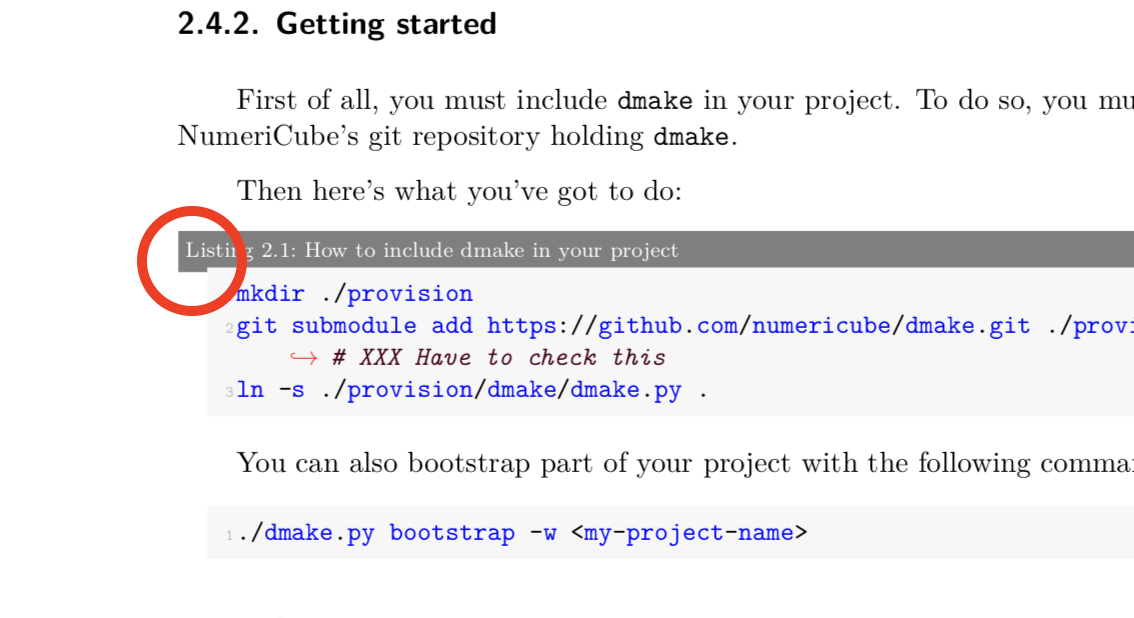
\includegraphics[width=\textwidth]{assets/alignmentpb.png}
\caption{Alignment problem}
\end{figure}
\end{lstlisting}

\subsection{Pretty boxes}

You can include pretty boxes with the \texttt{\textbackslash warningbox} directive.

\begin{lstlisting}[style=Latex-color]
\warningbox{This is a warning box.}
\end{lstlisting}

\warningbox{This is a warning box.}

For the record, here's the list of available boxes from the package:

\begin{lstlisting}[style=Latex-color]
\notebox{\lipsum[2]}
\tipbox{\lipsum[3]}
\warningbox{\lipsum[4]}
\cautionbox{\lipsum[5]}
\importantbox{\lipsum[6]}
\end{lstlisting}

\subsection{CSV files}

This is how to add a big CSV file.
\todo{Use the new format for tables (see \texttt{history.tex} file).}
For the record, this was generated with \texttt{git log \-\-date=local \-\-pretty=format:"\%h\%x09\%an\%x09\%ai\%x09\%s"}

\csvautolongtable[
    separator=tab,
    % no head,
    respect all
]{assets/commits.csv}
% {1=\hash,2=\author,3=\date,4=\comment}
% {\hash & \author & \date & \comment}


\section{Pretty schemas (using \texttt{TikZ})}

Ok let's admit it: drawing with \texttt{TikZ} in a complete abstract environment is a nightmare.

However, you can create a (free) account on \url{https://www.overleaf.com}, open the Drawing example
(\url{https://www.overleaf.com/latex/examples/hello-world-example/hthgmnnxbhhx}) and start fiddling
from there.

We provide a few examples of what we can do with styles included with the present document.

Figure \ref{figure:smpreleaseworkflow} provides an example of such a schema.

\begin{lstlisting}[style=Latex-color,caption={my-listing}]
\begin{figure}
\centering
\begin{tikzpicture}[node distance=2cm,
    every node/.style={fill=white, font=\sffamily}, align=center]
    \node (init)                [textbox0]
        {textbox0\\This is the textbox content};
    \node (write)               [textbox1, below of=init]
        {textbox1\\This is the textbox content};
    \node (testCode)            [textbox3, below of=write]
        {textbox3};
    \node (commitCode)          [textbox4, below of=testCode]
        {textbox4};
    \node (release)             [textbox1, below of=commitCode]
        {textbox5};
    \node (generate)            [textbox3, below of=release]
        {textbox3};

    \node (repeat) [right of=testCode,xshift=5cm]
           {Rinse, repeat};
    \draw[arrow]         (init) -- (write);
    \draw[arrow]         (write) -- (testCode);
    \draw[arrow]         (testCode) -- (commitCode);
    \draw[arrow]         (commitCode) -- (release);
    \draw[arrow]         (release) -- (generate);
    \draw[arrow]        (generate) -| (repeat);
    \draw[arrow]        (repeat) |- (init);
\end{tikzpicture}
\caption{Description of the overall release textbox1}
\label{figure:smpreleaseworkflow}
\end{figure}
\end{lstlisting}

% Workflow for development activites
\begin{figure}
\centering
\begin{tikzpicture}[node distance=2cm,
    every node/.style={fill=white, font=\sffamily}, align=center]
    \node (init)                [textbox0]
        {textbox0\\This is the textbox content};
    \node (write)               [textbox1, below of=init]
        {textbox1\\This is the textbox content};
    \node (testCode)            [textbox3, below of=write]
        {textbox3};
    \node (commitCode)          [textbox4, below of=testCode]
        {textbox4};
    \node (release)             [textbox1, below of=commitCode]
        {textbox5};
    \node (generate)            [textbox3, below of=release]
        {textbox3};

    \node (repeat) [right of=testCode,xshift=5cm]
           {Rinse, repeat};
    \draw[arrow]         (init) -- (write);
    \draw[arrow]         (write) -- (testCode);
    \draw[arrow]         (testCode) -- (commitCode);
    \draw[arrow]         (commitCode) -- (release);
    \draw[arrow]         (release) -- (generate);
    \draw[arrow]        (generate) -| (repeat);
    \draw[arrow]        (repeat) |- (init);
\end{tikzpicture}
\caption{Description of the overall release textbox1}
\label{figure:smpreleaseworkflow}
\end{figure}



% ISO 62304 activities
\begin{figure}
\centering
\begin{tikzpicture}[node distance=2cm,
    every node/.style={fill=white, font=\sffamily}, align=center]

    \node (section61)                [textbox1]
        {Software maintenance plan};
    \node (section62)               [textbox1, below of=section61]
        {Problem and modification analysis};
    \node (section53)            [textbox2, below of=section62]
        {Software architectural design};
    \node (section54)          [textbox1, below of=section53]
        {Software detailed design};
    \node (section55)             [textbox0, below of=section54]
        {Software unit implementation and verification};
    \node (section56)            [textbox1, below of=section55]
        {Software integration and integration testing};
    \node (section57)            [textbox3, below of=section56]
        {Software system testing};
    \node (section58)            [textbox1, below of=section57]
        {Software release};
    \draw[arrow]         (section61) -- (section62);
    \draw[arrow]         (section62) -- (section53);
    \draw[arrow]         (section53) -- (section54);
    \draw[arrow]         (section54) -- (section55);
    \draw[arrow]         (section55) -- (section56);
    \draw[arrow]         (section56) -- (section57);
    \draw[arrow]         (section57) -- (section58);

\end{tikzpicture}
\caption{Description of the overall release\\
\legendzero\ White dot that is used to show something that's white.\\
\legendone\ Same with a \texttt{textbox1} text, etc
}
\label{figure:smpreleaseworkflow}
\end{figure}


\section{Todo list}

If you ever need to mention things to do, use the following:

\begin{lstlisting}[style=Latex-color]
\todo{Thing not to forget}
\missingfigure{Figure you need to include}
\todo[inline]{An inline todo note}
\end{lstlisting}

With the default template, todos are automatically indexed at the end of your document.

\subsection{Miscellaneous stuff}

\begin{itemize}
    \item Change BW page to something like this \url{https://www.latextemplates.com/templates/books/2/book_2.pdf} (look at page 3)
    \item Add a backcover page (even if it's just white)
    \item Mention the excellent base template in acknoledgements: \url{https://github.com/jmrplens/TFG-TFM_EPS}
\end{itemize}

\subsection{Caption alignment error}

There's a slight alignment error with code captions when using \texttt{lstlisting} (see screenshot below). It has to be fixed.

\begin{figure}
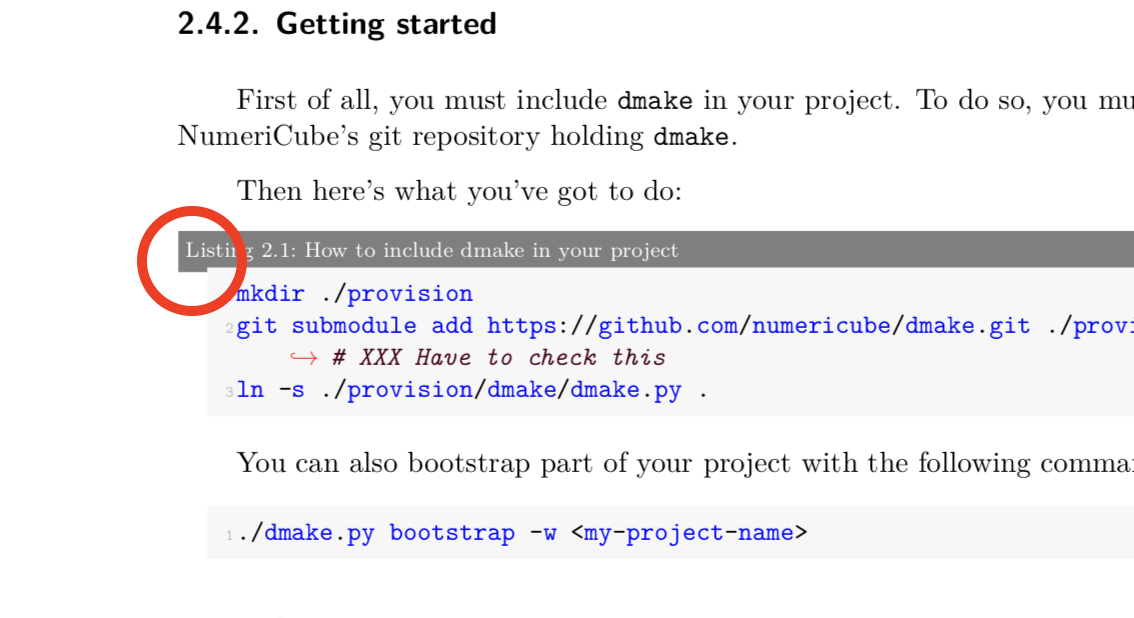
\includegraphics[width=\textwidth]{assets/alignmentpb.png}
\caption{Alignment problem}
\end{figure}


\subsection{Logos}

Logo management is far from perfect, especially on the front page (oops).

Probably need someone to make PDF-compliant EPS versions of my logo in various versions. See table \ref{table:logoformats} on page \pageref{table:logoformats} for a complete list of what we need.

\begin{table}[ht]
	\centering
	% {\scalefont{0.9}
	\begin{tabular}{@{}lccc@{}}
	\toprule
        Filename                        &   Baseline Language   &   Shape   & Base color \\ \midrule
        LogoN3-2018-EN-rect-white       &   English             & Rectangle & White/Transparent \\
        LogoN3-2018-FR-rect-white       &   French              & Rectangle & White/Transparent \\
        LogoN3-2018-EN-square-white     &   French              & Square    & White/Transparent \\
        LogoN3-2018-FR-square-white     &   French              & Square    & White/Transparent \\
        LogoN3-2018-EN-rect-black       &   English             & Rectangle & Black/Transparent \\
        LogoN3-2018-FR-rect-black       &   French              & Rectangle & Black/Transparent \\
        LogoN3-2018-EN-square-black     &   French              & Square    & Black/Transparent \\
        LogoN3-2018-FR-square-black     &   French              & Square    & Black/Transparent \\ \bottomrule
	\end{tabular}
	% }
	\caption{Different types of logos to have in the \texttt{include/logos} folder.}
	\label{table:logoformats}
\end{table}

\subsection{.gitignore}

We should document what should be in \texttt{.gitignore} (and not into git, then).

Ideas comming in mind:

\begin{itemize}
    \item \texttt{docgen} folder
    \item \texttt{build} folders
    \item \texttt{provision/history} folder (or maybe not?)
    \item \texttt{DS\_Store} Mac Finder folders
\end{itemize}

\section{Lorem ipsum (just to check text structure)}

\lipsum

%!TeX encoding = UTF-8
%!TeX root = ../main.tex
\chapter{Dataset Management}
\label{chapter:dataset-management}

This section explains how to manage and organize datasets for our various customers.

\section{Introduction}

The general rules for dataset management are these:

\begin{itemize}
    \item Data is stored in Microsoft Azure
    \item Data is stored as Azure File Share during working phase
    \item Data is stored in Azure blobs when frozen
    \item Access rights must be set:
    \begin{itemize}
        \item Per developer for general dataset management
        \item Per project for technical dataset access
    \end{itemize}
\end{itemize}

\section{Dataset storage management}

Here's the general outline.

\begin{enumerate}
    \item Create a storage account (and possibly a resource group) on Microsoft Azure
    \item Create a Blob and a FileShare called "dataset"
    \item Generate a SAS key for your customer
    \item Download Azure Storage Explorer (see \url{https://azure.microsoft.com/en-us/features/storage-explorer/})
    \item Use Azure Storage Explorer to get the SAS link as explained here: \url{https://blogs.msdn.microsoft.com/jpsanders/2017/10/12/easily-create-a-sas-to-download-a-file-from-azure-storage-using-azure-storage-explorer/}
    \item Transmit this information to your customer using \url{dead-drop.me}.
\end{enumerate}

\subsection{Create storage account from Azure}

\begin{itemize}
    \item Connect to Azure portal
    \item Go to "Storage accounts"
    \item Create an account for your customer\footnote{Use full lowercase for customer name}
    \item Don't forget to create a resource group for your customer\footnote{Use same capitalization as your customer's real name}
\end{itemize}


%!TeX encoding = UTF-8
%!TeX root = ../main.tex
\chapter{Dataset Management (user manual)}
\label{chapter:customer-dataset-management}

This chapter explains how to access your dataset folders in order to push (or retrieve) your data in NumeriCube's platform.

\section{Prerequisites}

Download and install Azure Storage Explorer from the following URL: \url{https://azure.microsoft.com/en-us/features/storage-explorer/}.

Azure Storage Explorer is available for \texttt{Windows}, \texttt{Mac OS X} and \texttt{Linux}.

Make sure you received a \texttt{dead-drop.me} link with a password. Use this link to copy in your clipboard the Azure Shared Access Signature URI that you will use to authenticate on the file server.

\section{File share configuration}

\begin{itemize}
    \item Install Azure Storage Explorer
    \item Fetch the Azure Shared Access Signature URI from the link you received from \texttt{dead-drop.me}.
    \item Open the Azure Storage Explorer application
    \item Click on the electrical plug on the left (see \ref{figure:az-step1})
        \begin{figure}
        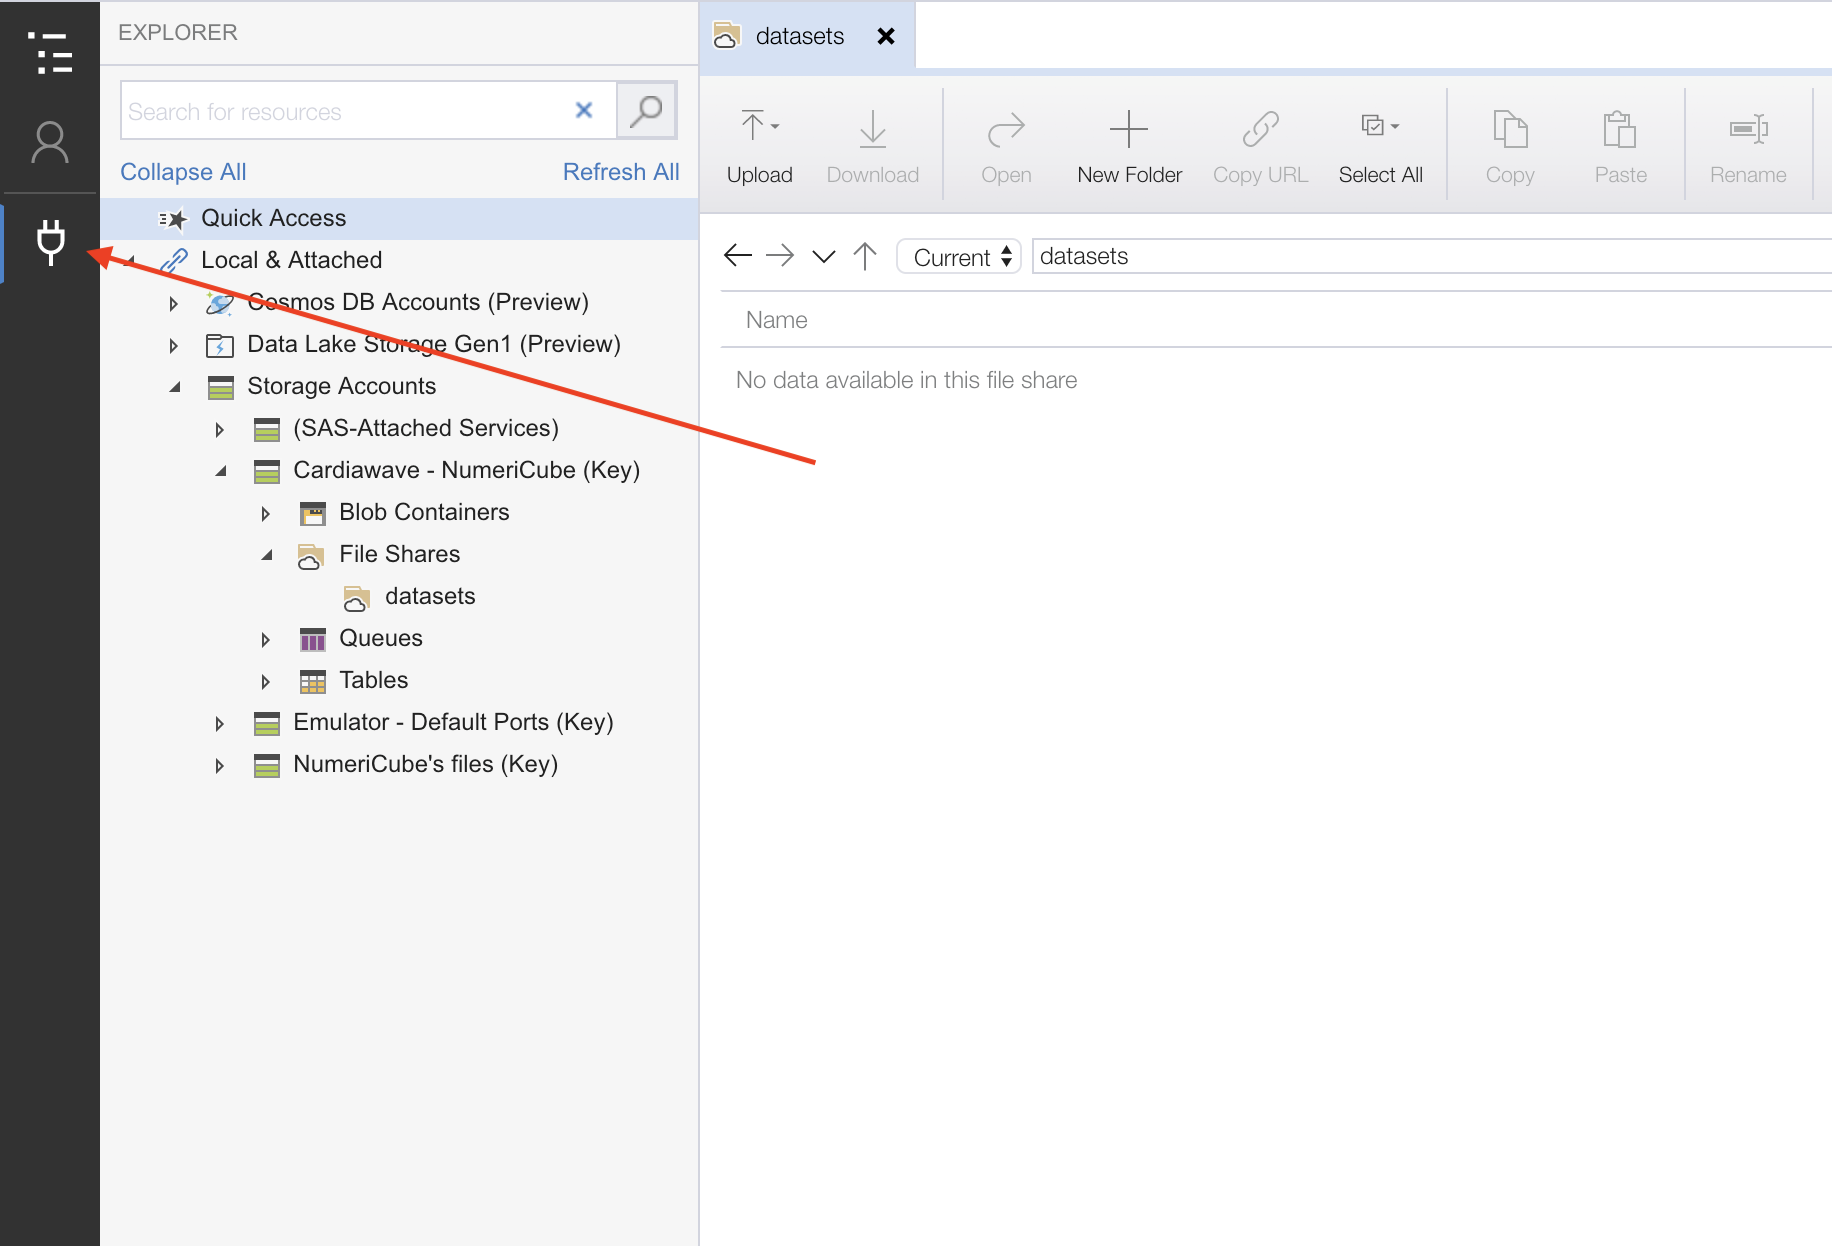
\includegraphics[width=\textwidth]{assets/az-step1.png}
        \caption{Connect to a new Azure file share}
        \label{figure:az-step1}
        \end{figure}
    \item Click the "Use Shared Access Signature URI" option and click \texttt{Next} (see \ref{figure:az-step2})
        \begin{figure}
        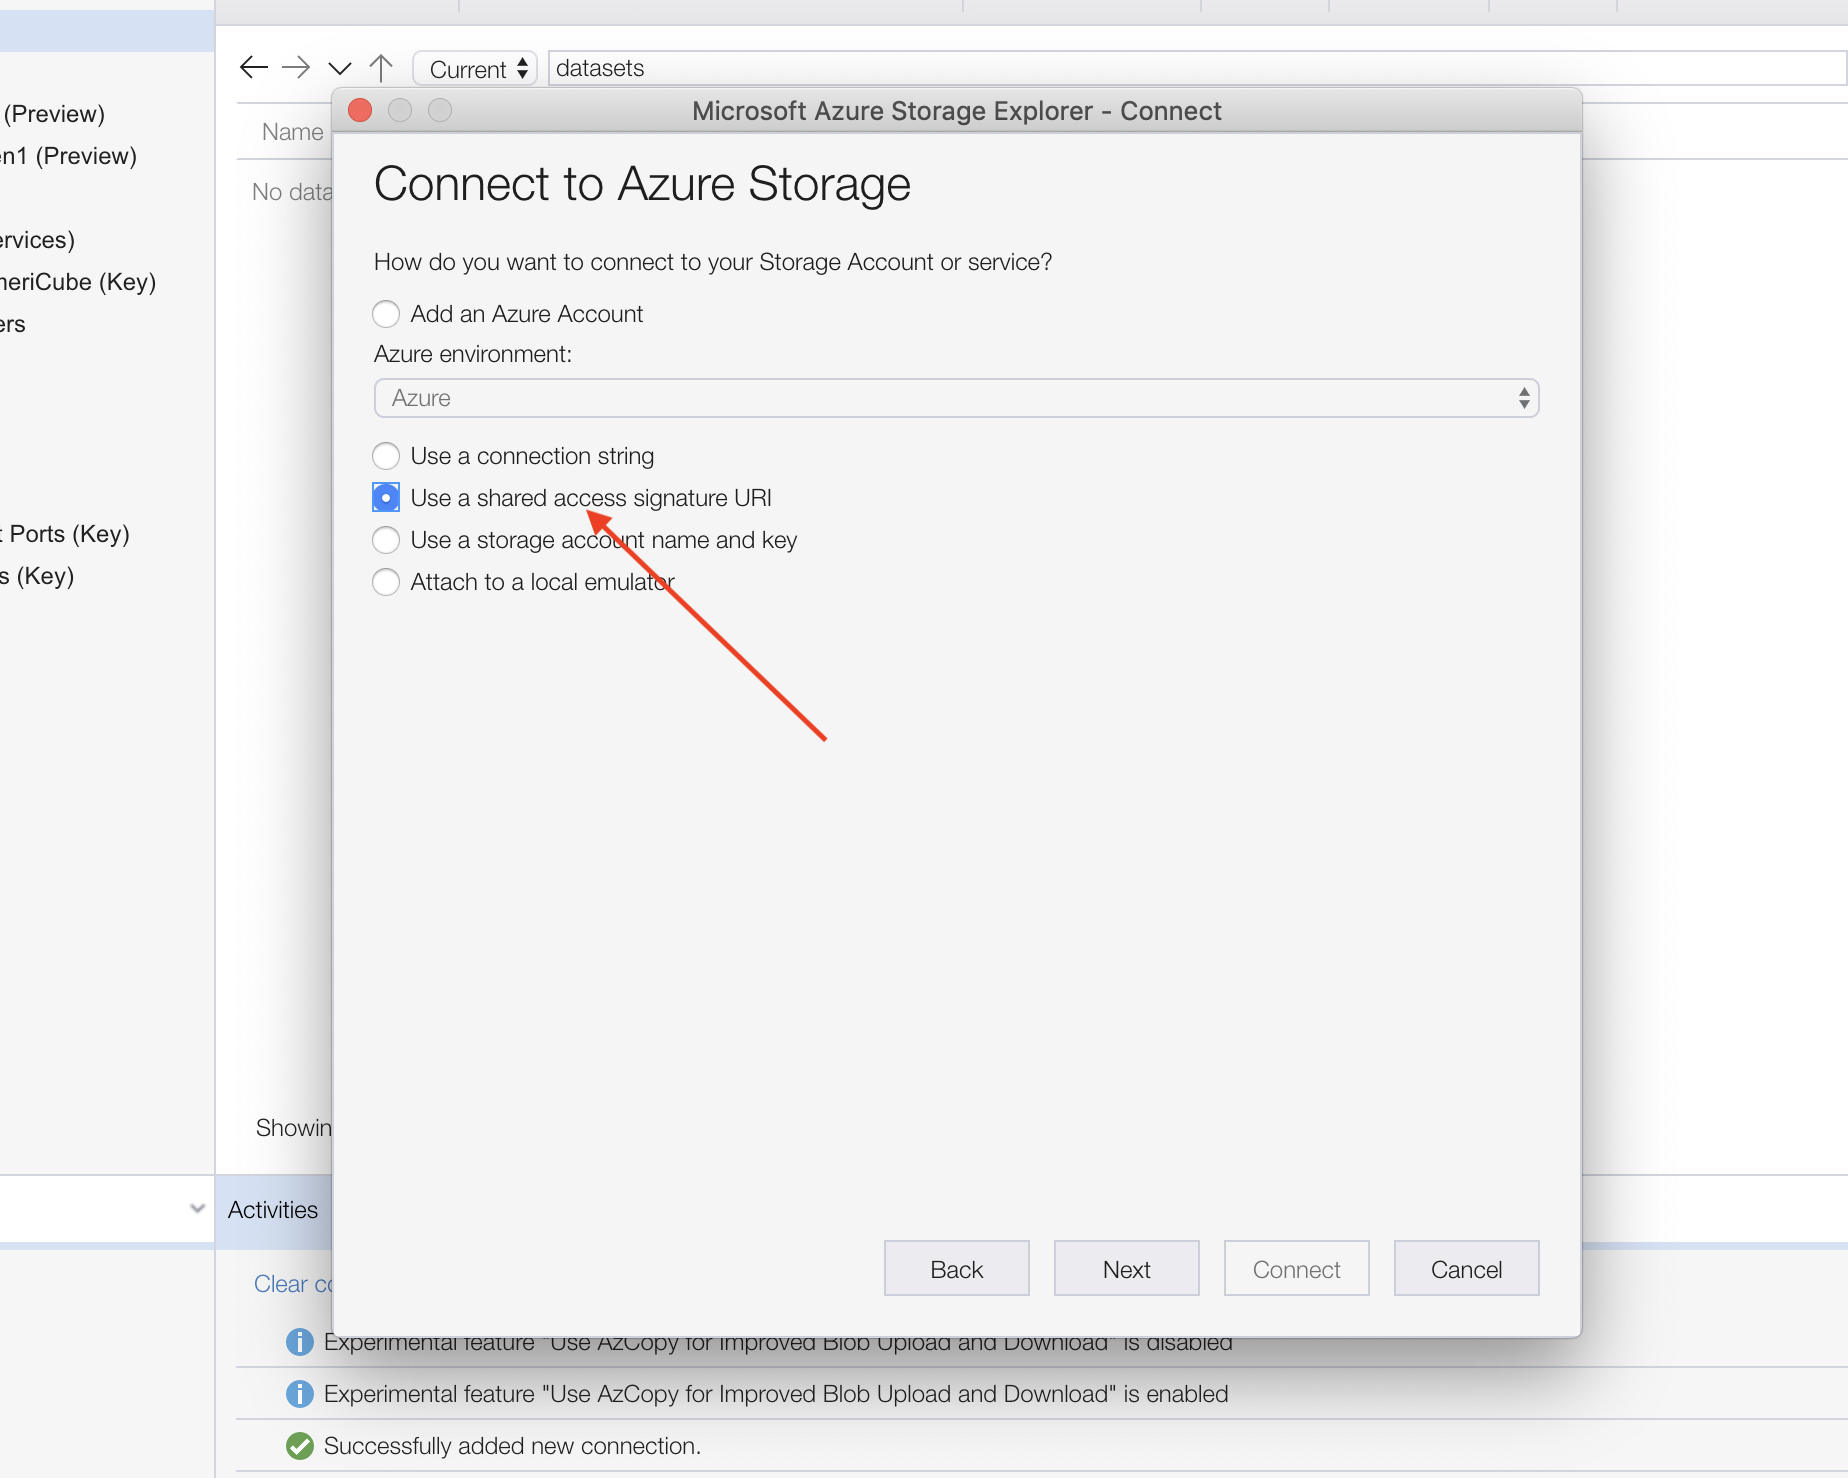
\includegraphics[width=\textwidth]{assets/az-step2.png}
        \caption{Connect to a new Azure file share}
        \label{figure:az-step2}
        \end{figure}
    \item Paste your Azure Shared Access Signature URI in the \texttt{URI} field and click \texttt{Next} (see \ref{figure:az-step3})
        \begin{figure}
        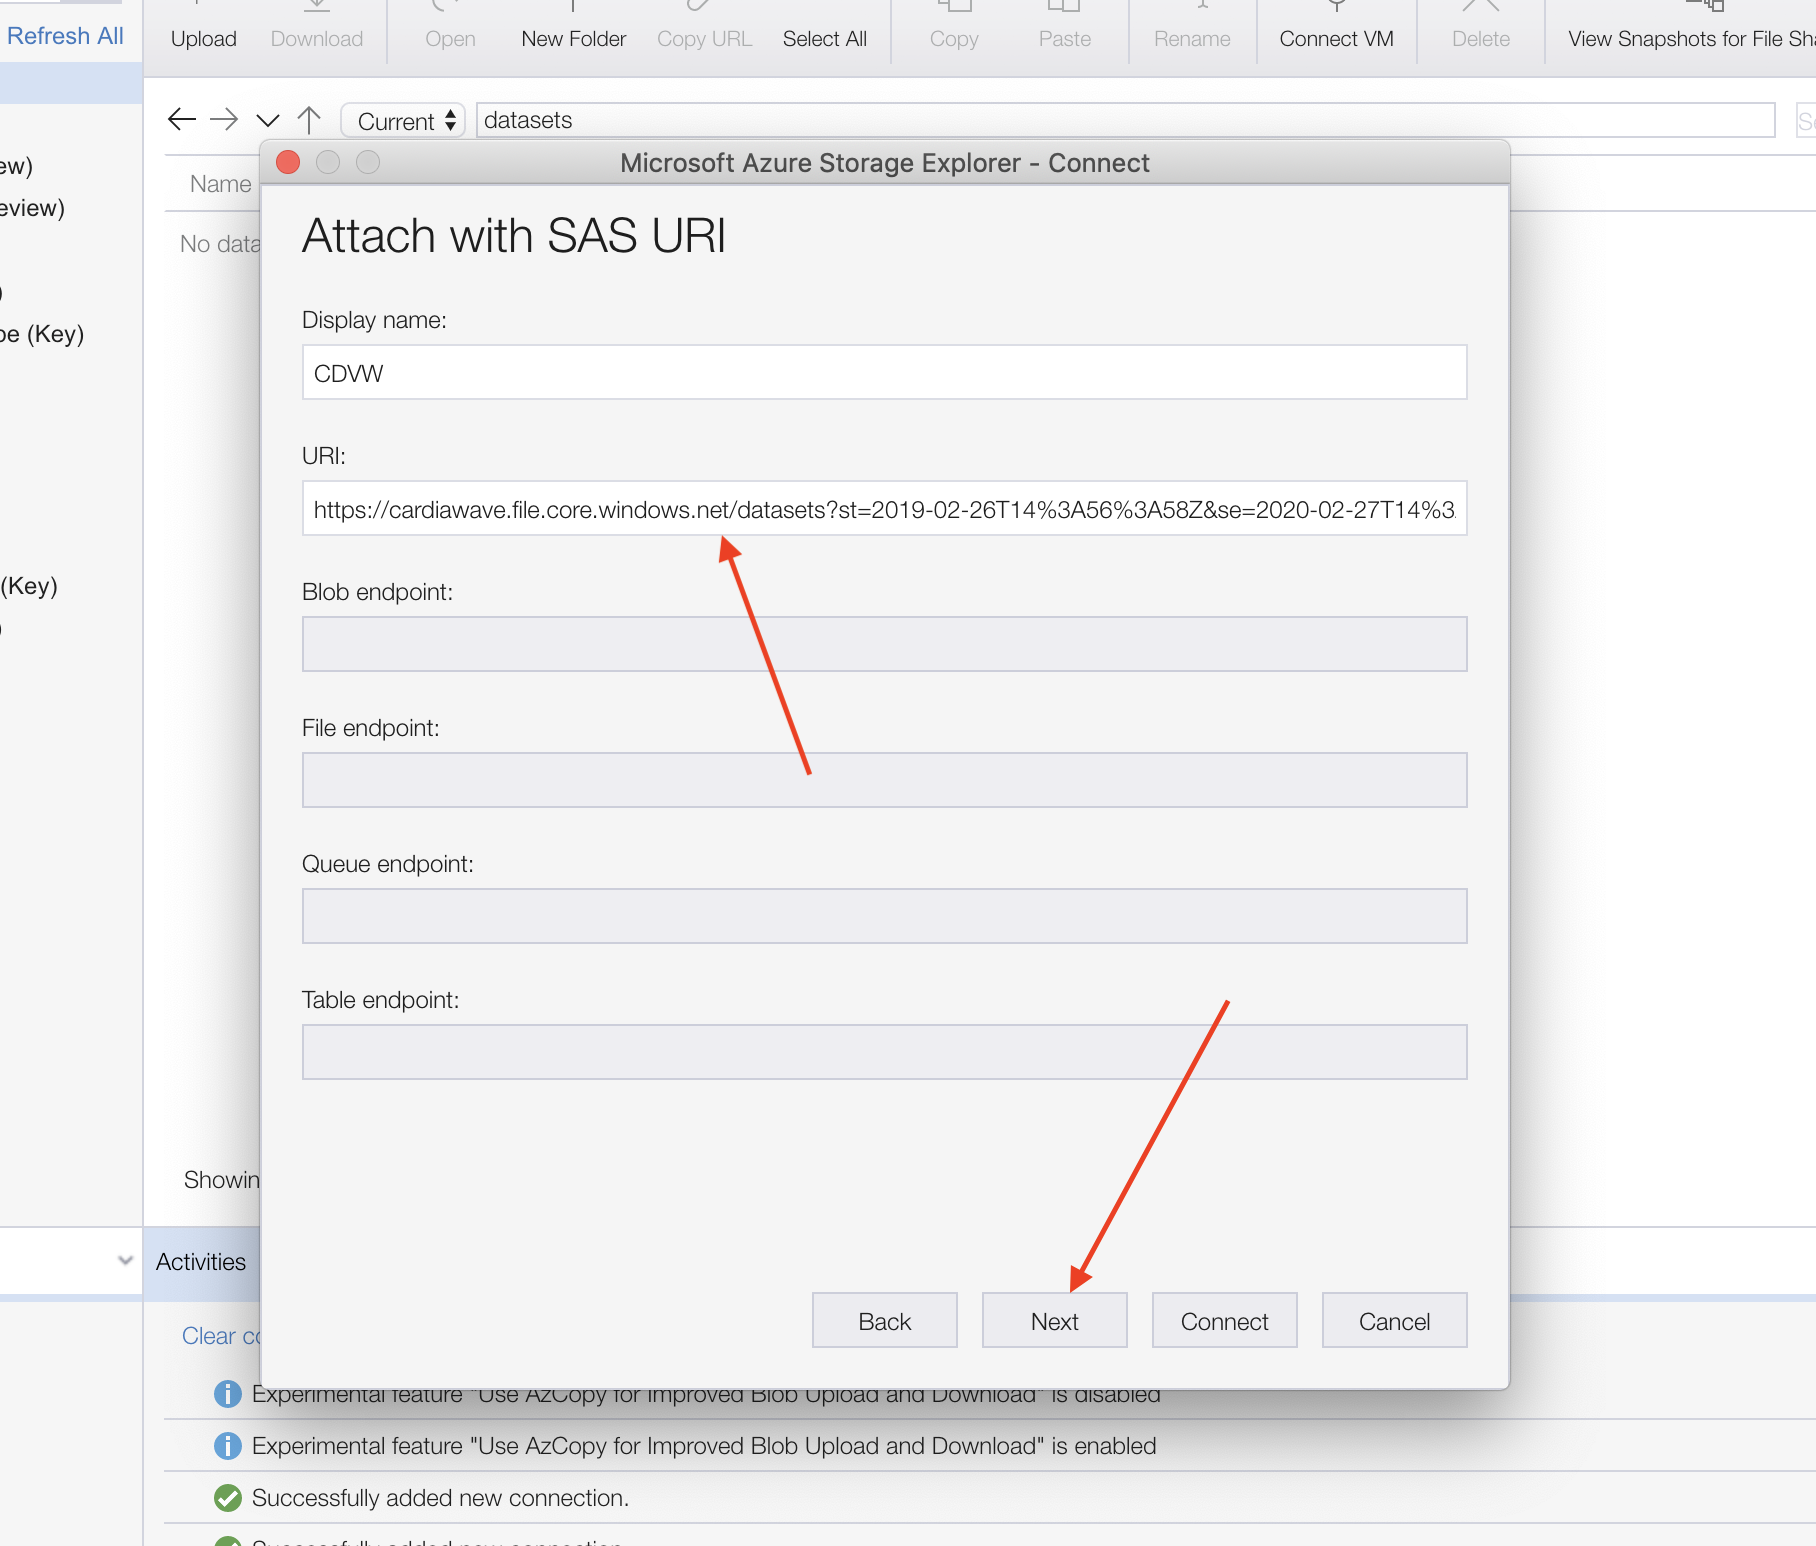
\includegraphics[width=\textwidth]{assets/az-step3.png}
        \caption{Connect to a new Azure file share}
        \label{figure:az-step3}
        \end{figure}
    \item Check the information, take note of the access expiration date and click \texttt{Connect} (see \ref{figure:az-step4})
        \begin{figure}
        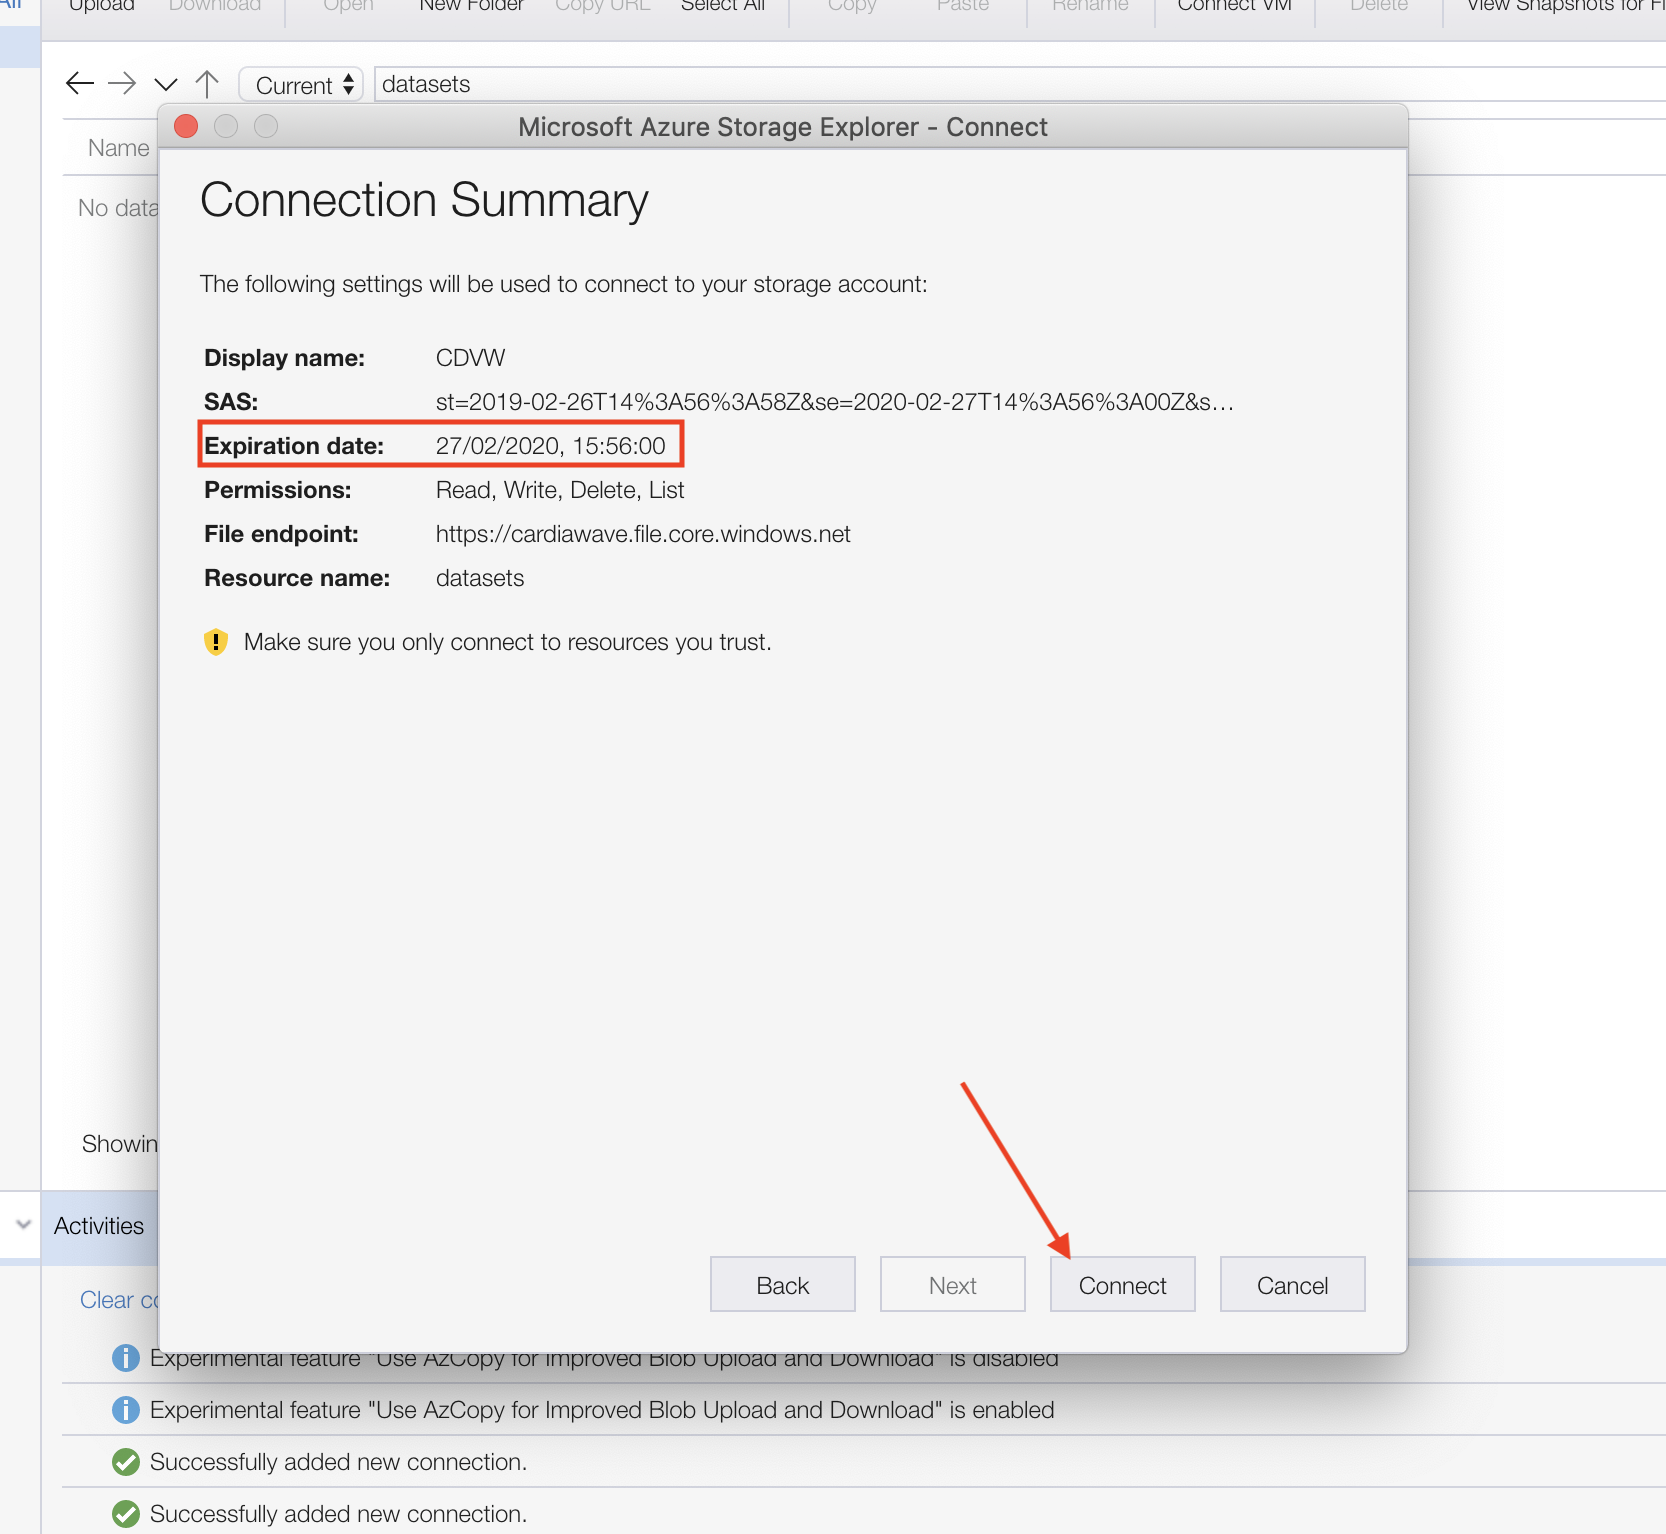
\includegraphics[width=\textwidth]{assets/az-step4.png}
        \caption{Connect to a new Azure file share}
        \label{figure:az-step4}
        \end{figure}
    \item That's it! You can use the explorer to drag and drop files to your file share, use the buttons to
    create folders, etc.
\end{itemize}

%!TeX encoding = UTF-8
%!TeX root = ../main.tex
\chapter{Additional documentation and must-read}
\label{chapter:must-read}

This section provides additional resources about critical parts of our projects.

It's aimed to be read by every maintainer on the project.

\section{General programming}

\begin{itemize}
    \item \href{https://www.joelonsoftware.com/2003/10/08/the-absolute-minimum-every-software-developer-absolutely-positively-must-know-about-unicode-and-character-sets-no-excuses/}{The absolute minimum one should know about Unicode}
\end{itemize}

\section{Docker}

\begin{itemize}
    \item \href{https://towardsdatascience.com/learn-enough-docker-to-be-useful-b7ba70caeb4b}{Learn enough Docker to be useful}
\end{itemize}

%!TeX encoding = UTF-8
%!TeX root = ../main.tex
\chapter{Sample Snap7 session}
\label{chapter:snap7}

This is an example of a successful Snap7 session.

\begin{lstlisting}[style=Python-color,caption={Sample Snap7 session}]
(ve_majurca) eurosilicone@eurosilicone-NUC8i3BEH:~/Bureau/majurca-ecoclassifier$ vi ve_majurca/lib/python3.6/site-packages/snap7/client.py
(ve_majurca) eurosilicone@eurosilicone-NUC8i3BEH:~/Bureau/majurca-ecoclassifier$ python
Python 3.6.7 (default, Oct 22 2018, 11:32:17)
[GCC 8.2.0] on linux
Type "help", "copyright", "credits" or "license" for more information.
>>> import snap7
>>> sn = snap7.client.Client()
>>> sn.connect('192.168.0.1', 0, 1)

# This is before PLC has been configured correctly
>>> sn.db_read(42, 0, 1)
b'CLI : function refused by CPU (Unknown error)'
Traceback (most recent call last):
  File "<stdin>", line 1, in <module>
  File "/home/eurosilicone/Bureau/majurca-ecoclassifier/ve_majurca/lib/python3.6/site-packages/snap7/client.py", line 145, in db_read
    check_error(result, context="client")
  File "/home/eurosilicone/Bureau/majurca-ecoclassifier/ve_majurca/lib/python3.6/site-packages/snap7/common.py", line 65, in check_error
    raise Snap7Exception(error)
snap7.snap7exceptions.Snap7Exception: b'CLI : function refused by CPU (Unknown error)'

# Ok, so now PLC is configured correctly, let's start again
>>> sn.disconnect()
>>> sn.connect('192.168.0.1', 0, 1)
>>> sn.db_read(43, 0, 1)
bytearray(b'\x00')
>>> sn.db_read(42, 0, 1)
b'CPU : Address out of range'
Traceback (most recent call last):
  File "<stdin>", line 1, in <module>
  File "/home/eurosilicone/Bureau/majurca-ecoclassifier/ve_majurca/lib/python3.6/site-packages/snap7/client.py", line 145, in db_read
    check_error(result, context="client")
  File "/home/eurosilicone/Bureau/majurca-ecoclassifier/ve_majurca/lib/python3.6/site-packages/snap7/common.py", line 65, in check_error
    raise Snap7Exception(error)
snap7.snap7exceptions.Snap7Exception: b'CPU : Address out of range'
>>> sn.db_read(43, 0, 1)
bytearray(b'\x00')
>>> sn.db_read(43, 0, 2)
bytearray(b'\x00+')
>>> sn.db_read(43, 0, 10)
b'CPU : Address out of range'
Traceback (most recent call last):
  File "<stdin>", line 1, in <module>
  File "/home/eurosilicone/Bureau/majurca-ecoclassifier/ve_majurca/lib/python3.6/site-packages/snap7/client.py", line 145, in db_read
    check_error(result, context="client")
  File "/home/eurosilicone/Bureau/majurca-ecoclassifier/ve_majurca/lib/python3.6/site-packages/snap7/common.py", line 65, in check_error
    raise Snap7Exception(error)
snap7.snap7exceptions.Snap7Exception: b'CPU : Address out of range'
>>> sn.db_read(43, 0, 8)
b'CPU : Address out of range'
Traceback (most recent call last):
  File "<stdin>", line 1, in <module>
  File "/home/eurosilicone/Bureau/majurca-ecoclassifier/ve_majurca/lib/python3.6/site-packages/snap7/client.py", line 145, in db_read
    check_error(result, context="client")
  File "/home/eurosilicone/Bureau/majurca-ecoclassifier/ve_majurca/lib/python3.6/site-packages/snap7/common.py", line 65, in check_error
    raise Snap7Exception(error)
snap7.snap7exceptions.Snap7Exception: b'CPU : Address out of range'
>>> sn.db_read(43, 0, 4)
bytearray(b'\x00+\x00,')
>>> ord(42)
Traceback (most recent call last):
  File "<stdin>", line 1, in <module>
TypeError: ord() expected string of length 1, but int found
>>> asc(43)
Traceback (most recent call last):
  File "<stdin>", line 1, in <module>
NameError: name 'asc' is not defined
>>> chr(43)
'+'
>>> ord(',')
44
>>> sn.db_write(43, 0, b'x')
>>> ord('x')
120
>>> sn.db_write(43, 0, b'\x00x')
>>>
\end{lstlisting}


\todototoc
\listoftodos

%%%%
% BIBLIOGRAPHY AND GLOSSARY
%%%%
\nocite{*} % Include ALL articles in bibliography even if not cited
\bibliography{bibliography} % Bibliography content
\bibliographystyle{apacite}

\printglossary[style=altlist,type=\acronymtype,title={Terms, definitions, and abbreviations}]
\glsaddallunused

\input{include/cover_back}

\end{document}
